\documentclass[conference]{IEEEtran}
\IEEEoverridecommandlockouts
% The preceding line is only needed to identify funding in the first footnote. If that is unneeded, please comment it out.
\usepackage{cite}
\usepackage{amsmath,amssymb,amsfonts}
\usepackage{algorithmic}
\usepackage{graphicx}
\usepackage{textcomp}
\usepackage{xcolor}
\usepackage{pgfplots}
\def\BibTeX{{\rm B\kern-.05em{\sc i\kern-.025em b}\kern-.08em
    T\kern-.1667em\lower.7ex\hbox{E}\kern-.125emX}}
\begin{document}

\title{Príncipios de Localidade na Cache: Impacto de Técnicas e Arquiteturas na Performance.\\

}

\author{\IEEEauthorblockN{Gabriel Araujo Campos Silva}
\IEEEauthorblockA{\textit{Pontifícia Universidade Católica de Minas Gerais}}
\and
\IEEEauthorblockN{Gabriel Rangel}
\IEEEauthorblockA{\textit{Pontifícia Universidade Católica de Minas Gerais}}}

\maketitle

\section{Introdução}
A memória cache é um componente de Hardware de computadores que armazena dados/instruções e tem rápido tempo de acesso, apesar de seu espaço ser reduzido. Para extrair o máximo de eficiência dessa memória, existem diversas técnicas capazes de otimizar sua performance.

A performance de uma memória Cache é medida através do cache miss, que é uma métrica para mensurar quantas vezes a informação que o processador necessita estava armazenada. É importante ressaltar que cada vez que um dado não é encontrado na Cache, ocorre um acesso às demais memórias, que consequentemente gastam mais tempos para fazer essa busca.

De acordo com Patterson e Hennessy \cite{patterson2017}, a localidade temporal é o princípio em que se um local de dados é referencado, então, ele tenderá aa ser referenciado novamente em breve. Enquanto a localidade espacial é o princípio em que, se um local de dados é referenciado, então, os próximos dados com endereços próximos tenderão a ser referenciados em breve.

Para explorar as os conceitos de localidade, existem diferentes arquiteturas que possibilitam mapear a memória de forma a diminuir ou aumentar a quantidade de substituições que serão feitas ao longo de uma execução. Além disso, os princípios também podem ser analisados de acordo com as políticas de substituição de um dado na memória. Por fim, o tamanho dos blocos e das palavras também interfere na performance e pode perturbar o melhor uso das localidades.

O trabalho apresenta a comparação entre algumas técnicas de substituição, como LRU (Least Recently Used) e FIFO (First In First Out), além de diferentes arquiteturas de memória, como Mapeamento Direto, Associativa por conjuntos e Completamente Associativa, e como cada alteração impacta o cache miss através de uma análise sobre o funcionamento de cada, comparação entre todass e simulação do funcionamento da memória através do simulador Amnesia.

\section{Trabalhos Correlatos}
Como embasamento desse trabalho, foram utilizados os seguintes artigos e pesquisas relacionadas:
\subsection{"Amnesia: um Objeto de Aprendizagem para o Ensino de Hierarquia de Memória" - Instituto de Ciências Matemáticas e de Computação – ICMC/USP}
Esse artigo explica o funcionamento do simulador Amnesia, ferramenta principal utilizada para testes de memória nesse trabalho. O documento aborda o projeto Amnesia e sua principal funcionalidade: permitir analisar o desempenhoi da hierarquia  de memória na arquitetura de Von Neumann, simulando desde o processador até as caches, memória principal e disco (caso o objeto de estudo seja a memória virtual). Esse artigo também apresenta um tutorial de como utilizar a ferramenta, além de resultados de estatísticas geradas pelo próprio simulador.

\subsection{"Avanços na Arquitetura de Memória Cache" - UNESP - IBILCE}
O artigo traz uma visão mais teórica a respeito da hierarquia de memória, dando ênfase em diversas arquiteturas reais de processadores e comparando a evolução das memórias ao longo do tempo. Não obstante, o trabalho apresenta um detalhamento teórico importante para o entendimento do processo de hierarquia de memória, além de oferecer embasamento teórico de conceitos importantes para essa pesquisa.

\subsection{"Aprendendo Hierarquia de Mem´oria e a Explorac¸˜aodas Localidades Espacial e Temporal com o Simulador Amnesia" - Pontif´ıcia Universidade Cat´olica de Minas Gerais}
O artigo aborda a importância do simulador Amnesia para o estudo da hierarquia de memória, e além disso, trabalha diversos conceitos essenciais para o entendimento do trabalho. Também apresenta pontos importantes para serem analisados no estudo da memória Cache, como tamanho da cache, tamanho do bloco por conjunto e níveis de associatividade. Além disso, sugere diversos casos de teste para o estudo da performance da memória e os devidos resultados, que foram utilizados como referência para pensar nos testes desse trabalho.

Além das pesquisas e artigos citados acima, outras referências foram utilizadas principalmente para melhorar o entendimento de conceitos teóricos como localidade espacial e temporal, e com isso, refinar os testes e resultados desse trabalho.

\section{Metodologia}
Para o desenvolvimento desse trabalho, adotamos algumas etapas importantes, afim de garantir a qualidade das informações e o entendimento do conteúdo por todos os membros do grupo. Em primeiro lugar, artigos relacionados foram levantados, assim como bibliografias de maior tamanho, e após a leitura de todo o material, os principais são utilizados como referências nessa pesquisa.

Após o entendimento do conteúdo que seria abordado, foi realizado um estudo sobre o funcionamento do simulador Amnesia. O simulador utiliza dois componentes principais para gerar os dados necessários para o trabalho: arquitetura e trace. A arquitetura do processador é passada ao simulador por meio de um arquivo XML, e possui os seguintes campos:

\begin{table}[h!]
\centering
\begin{tabular}{|l|}
\hline
\textbf{Campo} \\ \hline
processorContains \\ \hline
createTraceFile \\ \hline
wordSize (Trace) \\ \hline
wordSize (CPU) \\ \hline
blockSize \\ \hline
memorySize (MainMemory) \\ \hline
ciclesPerAccessRead (MainMemory) \\ \hline
ciclesPerAccessWrite (MainMemory) \\ \hline
timeCicle (MainMemory) \\ \hline
cacheType \\ \hline
lineSize \\ \hline
ciclesPerAccessRead (Cache) \\ \hline
ciclesPerAccessWrite (Cache) \\ \hline
timeCicle (Cache) \\ \hline
memorySize (Cache) \\ \hline
associativityLevel \\ \hline
writePolicy \\ \hline
replacementAlgorithm (Cache) \\ \hline
pageSize \\ \hline
diskMemorySize \\ \hline
diskCiclesPerAccessRead \\ \hline
diskCiclesPerAccessWrite \\ \hline
timeCicle (VirtualMemory) \\ \hline
pageTableReplacementAlgorithm \\ \hline
TLBType \\ \hline
memorySize (TLB) \\ \hline
ciclesPerAccessRead (TLB) \\ \hline
ciclesPerAccessWrite (TLB) \\ \hline
timeCicle (TLB) \\ \hline
replacementAlgorithm (TLB) \\ \hline
\end{tabular}
\caption{Campos do XML}
\label{tab:xmlcampos}
\end{table}

Sendo que cada campo é uma característica da memória que pode ser alterada a fim de validar alguma hipótese e realizar os testes. Por exemplo, o campo replacementAlgorithm diz respeito a política de substituição no caso de algum conflito de endereços na Cache.

Já o arquivo de trace é responsável por testar a arquitetura proposta, contendo acessos realizados por um programa à memória, acessos de leitura, escrita de dados ou busca de instruções. O mesmo é composto por várias linhas, sendo que cada uma contém um rótulo(decimal) e um endereço(hexadecimal). Através do arquivo de traço é possível gerar estatísticas sobre a memória.

\begin{table}[h!]
\centering
\begin{tabular}{lll}
\hline
\multicolumn{3}{l}{\textbf{Trace 1}} \\ \hline
2 & 5 & // busca de instrução no endereço 5 \\ 
2 & c & // busca de instrução no endereço c \\ 
2 & b & // busca de instrução no endereço b \\ 
2 & a & // busca de instrução no endereço a \\ 
2 & f & // busca de instrução no endereço f \\ 
2 & 8 & // busca de instrução no endereço 8 \\ 
2 & 0 & // busca de instrução no endereço 0 \\ 
2 & 9 & // busca de instrução no endereço 9 \\ 
2 & 4 & // busca de instrução no endereço 4 \\ 
2 & 1 & // busca de instrução no endereço 1 \\ \hline
\end{tabular}
\caption{Exemplo de Trace}
\label{tab:traceAleatorio}
\end{table}

Após o entendimento de como utilizar a ferrmamenta, foram traçados alguns casos de teste que comparam resultados para identificar quais as melhores configurações para a memória para que alcance a melhor pertformance dado uma séria de requisitos.

\subsection{Caso de Teste 1 - Melhor arquitetura dado o tamanho dos blocos}
Afim de explorar a localidade espacial, o objetivo é testar todas as formas de organizar a memória com mesmos tamanhos de blocos, afim de identificar qual é a melhor para blocos muito grandes (ou se a performance é afetada para todas).

\subsection{Caso de Teste 2 - Impacto do aumento da associatividade na memória}
Nesse teste, o objetivo é aumentar gradativamente a associatividade da cache de N conjuntos, sendo N o número de blocos até 1 conjunto, observando o impacto na performance.

\subsection{Caso de Teste 3 - Impacto do tamanho dos blocos em cada modelo de organização}
Complementar ao Caso de Teste 1, o objetivo desse experimento é analisar individualmente cada uma das formas de orgaizar a cache e entender o impacto na performance na medida que aumentamos o tamanho dos blocos.

\subsection{Caso de Teste 4 - Melhor política de substituição para cada arquitetura}
Afim de analisar os conflitos na Cache, esse teste visa testar algumas políticas de substituição individualmente em cada arquitetura e definir qual se aplica melhor em cada uma delas.

A partir desses testes, será possível comparar os resultados de performance, cache miss entre outras métricas afim de chegar em conclusões importantes sobre a exploração das localidades em cada ponto da arquitetura na hora de projetar uma hierarquia de memória.


\section{Arquiteturas Propostas}
Com os casos de teste definidos, é possível projetar as arquiteturas de cada um dos testes, assim como quais propriedades serão constantes em cada teste, quais propriedades se alteram e quais métricas são utilizadas para obter os resultados e conclusões. Afim de não poluir o trabalho, apenas as propriedades constantes e que se alteram serão citadas, enquanto as arquiteturas e traces completos podem ser encontrados no repositório do trabalho.

\subsection{Primeira variação de arquitetura}
O primeiro teste tem como intuito identificar qual forma de organização da memória cache (Mapeamento direto, Associativo por conjunto e Completamente Associativo) se comporta melhor com o aumento do tamanho dos blocos.

\begin{table}[htb]
\centering
\begin{tabular}{|l|l|}
\hline
\textbf{Propriedade}       & \textbf{Valores}         \\ \hline
Tamanho da Cache           & 256B                    \\ \hline
Organização                & M.D*, A.C*, C.A*        \\ \hline
Tamanho da Palavra         & 4B                  \\ \hline
Palavras por Bloco         & 4, 8, 16                \\ \hline
Quantidade de Blocos       & 16, 8 e 4           \\ \hline
Tamanho do Conjunto        & 4 blocos (Para A.C*)    \\ \hline
\end{tabular}
\caption{Propriedades Fixas e Varíaveis das arquiteturas do primeiro caso de teste}
\label{tab:propriedades}
\vspace{0.5cm}
\footnotesize
\textbf{Legenda:} M.D = Mapeamento Direto, A.C = Associativo por Conjunto, C.A = Completamente Associativo.
\end{table}

\subsection{Segunda variação de arquitetura}
O segundo teste visa observar o impacto do aumento da associatividade na performance da cache, portanto, o tamanho de blocos por conjunto é aumentado gradativamente para analisar as estatísticas.

\begin{table}[htb]
\centering
\begin{tabular}{|l|l|}
\hline
\textbf{Propriedade}       & \textbf{Valores}         \\ \hline
Tamanho da Cache           & 256B                    \\ \hline
Organização                & Assoc. por Conjunto        \\ \hline
Tamanho da Palavra         & 4B                  \\ \hline
Palavras por Bloco         & 2                \\ \hline
Quantidade de Blocos       & 32          \\ \hline
Tamanho do Conjunto        & 4, 8, 16, 32    \\ \hline
\end{tabular}
\caption{Propriedades Fixas e Varíaveis das arquiteturas do segundo caso de teste}
\label{tab:propriedades}
\vspace{0,5 cm}
\end{table}

\subsection{Terceira variação da arquitetura}
Complementar ao primeiro caso de teste, o objetivo é visualizar para cada nível de associatividade individualmente, como o aumento do bloco se comporta.

\begin{table}[htb]
\centering
\begin{tabular}{|l|l|}
\hline
\textbf{Propriedade}       & \textbf{Valores}         \\ \hline
Tamanho da Cache           & 256B                    \\ \hline
Organização                & M.D*, A.C*, C.A*        \\ \hline
Tamanho da Palavra         & 4B                  \\ \hline
Palavras por Bloco         & 4, 8, 16                \\ \hline
Quantidade de Blocos       & 16, 8 e 4           \\ \hline
Tamanho do Conjunto        & 4 blocos (Para A.C*)    \\ \hline
\end{tabular}
\caption{Propriedades Fixas e Varíaveis das arquiteturas do terceiro caso de teste}
\label{tab:propriedades}
\vspace{0.5cm}
\footnotesize
\textbf{Legenda:} M.D = Mapeamento Direto, A.C = Associativo por Conjunto, C.A = Completamente Associativo.
\end{table}

\subsection{Quarta variação de arquitetura}
O objetivo desse teste é comparar as duas políticas de substituição permitidas pelo simulador: LRU e FIFO. Para isso, cada uma foi aplicada em cada forma de organização para observar sua performance como um todo e qual a interferência do nível de associatividade.

\begin{table}[htb]
\centering
\begin{tabular}{|l|l|}
\hline
\textbf{Propriedade}       & \textbf{Valores}         \\ \hline
Tamanho da Cache           & 256B                    \\ \hline
Organização                & M.D*, A.C*, C.A*        \\ \hline
Tamanho da Palavra         & 4B                  \\ \hline
Palavras por Bloco         & 2                \\ \hline
Quantidade de Blocos       & 32         \\ \hline
Tamanho do Conjunto        & 4 blocos (Para A.C*)    \\ \hline
Substituição               & LRU, FIFO \\ \hline
\end{tabular}
\caption{Propriedades Fixas e Varíaveis das arquiteturas do quarto caso de teste}
\label{tab:propriedades}
\vspace{0.5cm}
\footnotesize
\textbf{Legenda:} M.D = Mapeamento Direto, A.C = Associativo por Conjunto, C.A = Completamente Associativo.
\end{table}

\section{Avaliação dos Resultados}
Nessa seção, os resultados dos testes realizados anteriormente são comparados e interpretados afim de reunir embasamento suficiente para obter as conclusões propostas. Para cada teste, as arquiteturas citadas anteriormente foram testadas com 5 traces diferentes, variando o número e a ordem de operações de leitura e escrita na memória, porém respeitando uma proporção de COMPLETAR-PÓS-ESCREVER-TRACES.

\subsection{Impacto do Tamanho dos Blocos no Cache Hit}
Após 4 iterações com traces de tamanhos e informações variáveis, foi possível chegar nos seguintes resultados:

\begin{table}[h!]
\centering
\renewcommand{\arraystretch}{1.5}
\setlength{\tabcolsep}{5pt}
\begin{tabular}{|c|c|c|c|c|}
\hline
\textbf{Organização} & \textbf{T. Bloco} & \textbf{Cache Hit} \\ \hline
Map. Direto              & 16B               & 0,77            \\ \hline
Map. Direto              & 32B               & 0,86           \\ \hline
Map. Direto              & 64B                 & 0,9            \\ \hline
A. Por Conjunto          & 16B                & 0,72            \\ \hline
A. Por Conjunto          & 32B               & 0,85            \\ \hline
A. Por Conjunto          & 64B                & 0,87            \\ \hline
C. Associativo           & 16B               & 0,77            \\ \hline
C. Associativo           & 32B                & 0,83            \\ \hline
C. Associativo           & 64B                & 0,80            \\ \hline
\end{tabular}
\caption{Tabela de Resultados Primeiro Teste}
\label{tab:media_final}
\end{table}

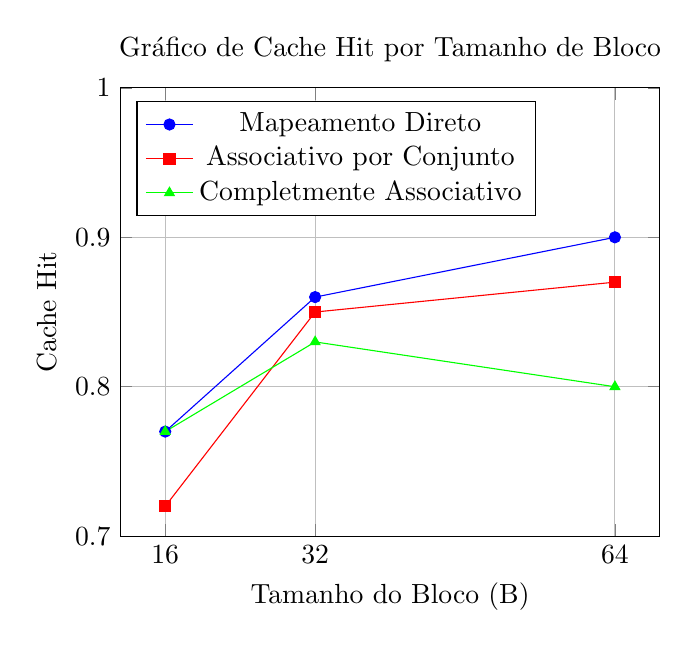
\begin{tikzpicture}
\begin{axis}[
    xlabel={Tamanho do Bloco (B)},
    ylabel={Cache Hit},
    xtick={16,32,64},
    legend pos=north west,
    grid=major,
    ymin=0.7, ymax=1,
    title={Gráfico de Cache Hit por Tamanho de Bloco},
]

% Linha 1
\addplot[color=blue,mark=*] coordinates {
    (16,0.77)
    (32,0.86)
    (64,0.9)
};
\addlegendentry{Mapeamento Direto}

% Linha 2
\addplot[color=red,mark=square*] coordinates {
    (16,0.72)
    (32,0.85)
    (64,0.87)
};
\addlegendentry{Associativo por Conjunto}

% Linha 3
\addplot[color=green,mark=triangle*] coordinates {
    (16,0.77)
    (32,0.83)
    (64,0.8)
};
\addlegendentry{Completmente Associativo}

\end{axis}
\end{tikzpicture}

A partir dos resultados é possível observar que o aumento dos blocos acaba diminuindo a performance da cache, já que, apesar de explorar as localidades pois obtém mais blocos contíguos da memória principal, consequentemente o número de linhas/conjuntos é reduzido, fazendo com que menos endereços de memória possam ser mapeados simultaneamente, forçando maior número de substituições e diminuindo o cache hit.

É possível observar também que, a cache com mapeamento direto se sobresai em todos os tamanhos de bloco, enquanto as caches associativas tem uma performance um pouco inferior. A cache completamente associativa, a partir do tamanho de 32 Bytes já apresenta uma queda na performance, visto que possui um conjunto por blocos, e com cada bloco contendo 16 palavras faz com que a cache só tenha 
4 conjuntos.

Logo, é possível concluir que o aumento do tamanho do bloco é positivo nas 3 arquiteturas até um certo ponto, no caso desse trabalho, de 32 bytes, ao qual passa a perder sua eficiência refletindo diretamente no cache hit analisado.

\subsection{Impacto da Associatividade no Cache Hit}
Os resultados da comparação variando o numero de conjuntos de uma cache associativa por conjunto mostram que o aumento dos conjuntos impacta positivamente a performance no geral.

Ao aumentar a associatividade, os miss hits por conflito diminuem, pois endereços que antes competiam pelo mesmo conjunto agora podem ser mapeados para conjuntos diferentes.

É importante ressaltar também que, ao aumentar demais o número dos conjuntos enquanto o tamanho da cache continua o mesmo diminui a associatividade da memória, resultando no aumento dos conflitos por capacidade caso o programa precise de mais blocos do que o número de blocos disponíveis em um conjunto, como mostra o gráfico no ponto em que o tamanho do conjunto é aumentado para 32 blocos.

\begin{table}[h!]
\centering
\renewcommand{\arraystretch}{1.5}
\setlength{\tabcolsep}{5pt}
\begin{tabular}{|c|c|c|c|c|}
\hline
\textbf{Organização} & \textbf{T. Conjunto} & \textbf{Cache Hit} \\ \hline
A. Por Conjuntos         & 4 Blocos                 & 0,62            \\ \hline
A. Por Conjunto          & 16 Blocos                & 0,71            \\ \hline
A. Por Conjunto          & 32 Blocos               & 0,78            \\ \hline
A. Por Conjunto          & 64 Blocos                & 0,72            \\ \hline
\hline
\end{tabular}
\caption{Tabela de Resultados Se Teste}
\label{tab:media_final}
\end{table}

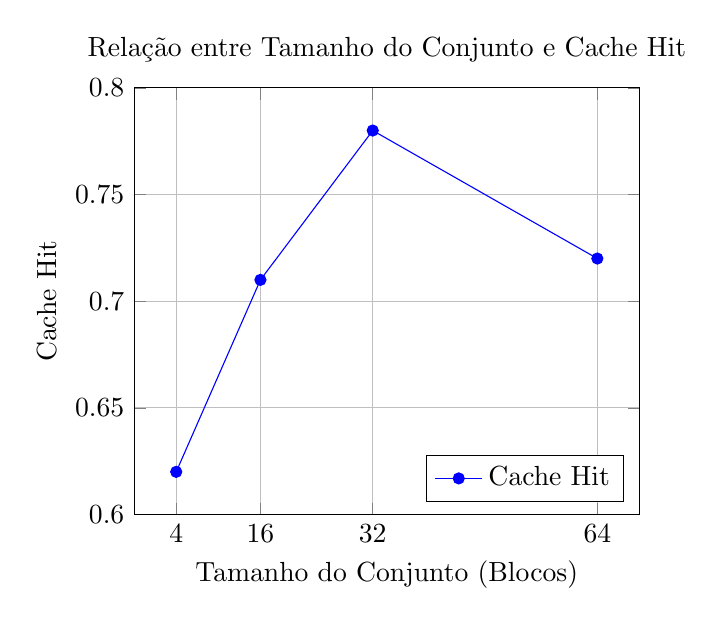
\begin{tikzpicture}
 \begin{axis}[
     xlabel={Tamanho do Conjunto (Blocos)},
     ylabel={Cache Hit},
     xtick=data,
     ymin=0.6, ymax=0.8,
     grid=major,
     width=8cm,
     height=7cm,
     legend pos=south east,
     title={Relação entre Tamanho do Conjunto e Cache Hit}
 ]
 % Dados da tabela
 \addplot[color=blue,mark=*] coordinates {
     (4, 0.62)
     (16, 0.71)
     (32, 0.78)
     (64, 0.72)
 };
 \legend{Cache Hit}
 \end{axis}
\end{tikzpicture}

\subsection{Ánálise Individual do Aumento de Blocos em Cada Arquitetura}
Complementar ao primeiro teste, a partir dos gráficos gerados nessa seção é possível entender melhor o impacto do aumento dos blocos em cada uma das arquiteturas de organização da memória.

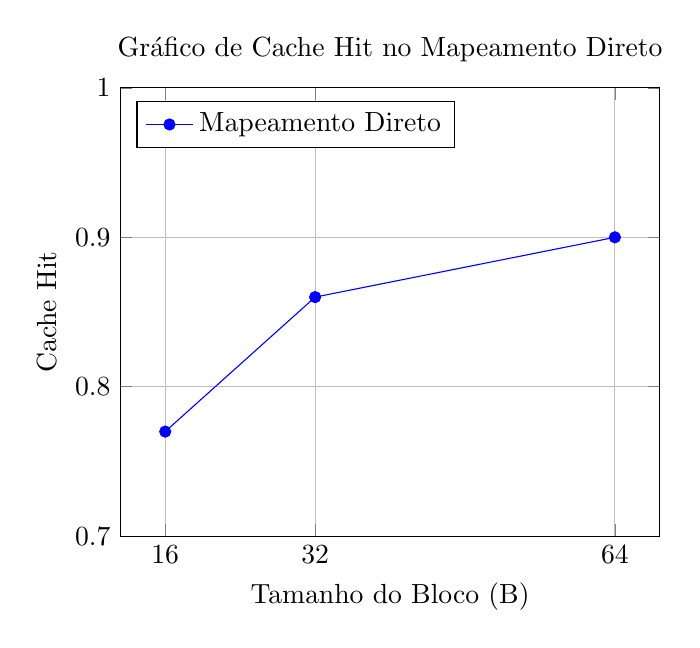
\begin{tikzpicture}
\begin{axis}[
    xlabel={Tamanho do Bloco (B)},
    ylabel={Cache Hit},
    xtick={16,32,64},
    legend pos=north west,
    grid=major,
    ymin=0.7, ymax=1,
    title={Gráfico de Cache Hit no Mapeamento Direto},
]

\addplot[color=blue,mark=*] coordinates {
    (16,0.77)
    (32,0.86)
    (64,0.9)
};
\addlegendentry{Mapeamento Direto}
\end{axis}
\end{tikzpicture}

No mapeamento direto, o aumento dos blocos significa que mais dados contíguos na memória principal serão trazidos para a Cache, e além disso, ocorre a redução de misses compulsórios. Porém, esse aumento também causa uma maior taxa de conflitos pois mais endereços de memória terão que ser mapeados para menos linhas, já que ao aumentar o tamanho do bloco sem aumentar o tamanho da cache, diminui o tamanho de linhas.

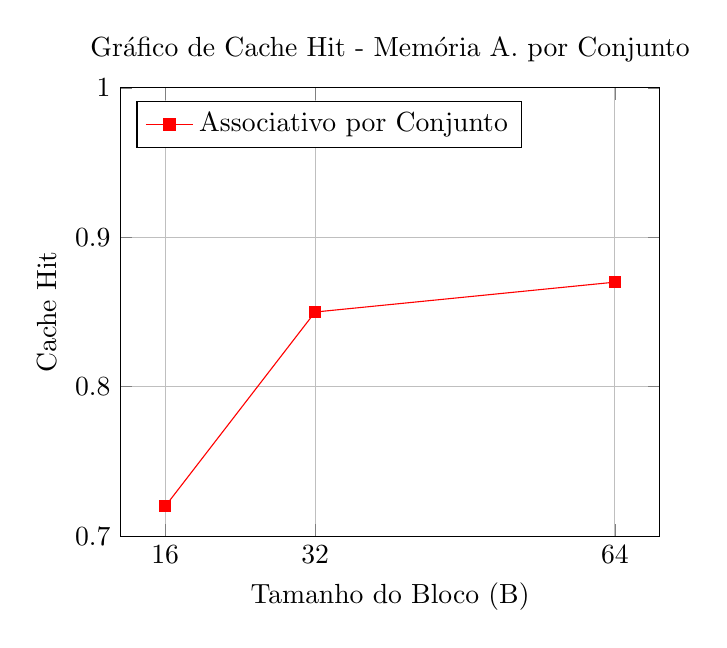
\begin{tikzpicture}
\begin{axis}[
    xlabel={Tamanho do Bloco (B)},
    ylabel={Cache Hit},
    xtick={16,32,64},
    legend pos=north west,
    grid=major,
    ymin=0.7, ymax=1,
    title={Gráfico de Cache Hit - Memória A. por Conjunto},
]
% Linha 2
\addplot[color=red,mark=square*] coordinates {
    (16,0.72)
    (32,0.85)
    (64,0.87)
};
\addlegendentry{Associativo por Conjunto}
\end{axis}
\end{tikzpicture}

Ao inserir a associatividade na memória, é perceptível que ocorre a redução de misses compulsórios e aumento do cache hit. Porém ao aumentar o tamanho dos blocos, o número de conjuntos também diminui, já que, ao aumentar o tamanho dos blocos sem aumentar o tamanho das caches, com uma associatividade N, a quantidade de conjuntos diminui,

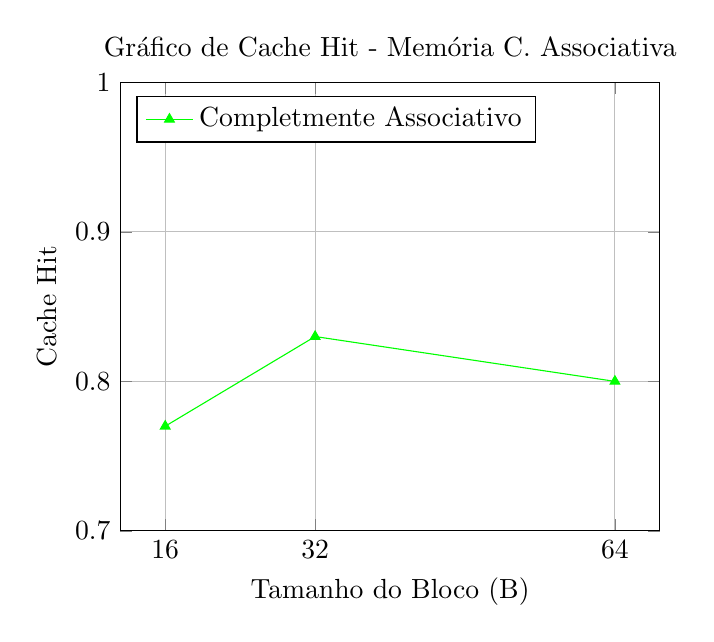
\begin{tikzpicture}
\begin{axis}[
    xlabel={Tamanho do Bloco (B)},
    ylabel={Cache Hit},
    xtick={16,32,64},
    legend pos=north west,
    grid=major,
    ymin=0.7, ymax=1,
    title={Gráfico de Cache Hit - Memória C. Associativa},
]
% Linha 3
\addplot[color=green,mark=triangle*] coordinates {
    (16,0.77)
    (32,0.83)
    (64,0.8)
};
\addlegendentry{Completmente Associativo}
\end{axis}
\end{tikzpicture}

O nível máximo de associatividade traz problemas semelhantes ao anterior, já que, quanto maior o bloco, menos conjuntos a cache terá, pois nessa arquitetura, existe sempre um bloco por conjunto. Além disso, é possível identificar que essa arquitetura é mais sensível ao aumento do bloco, já que apresenta uma queda na performance bem maior do que as outras arquiteturas.

\subsection{Análise das Políticas de Substituição por Arquitetura}

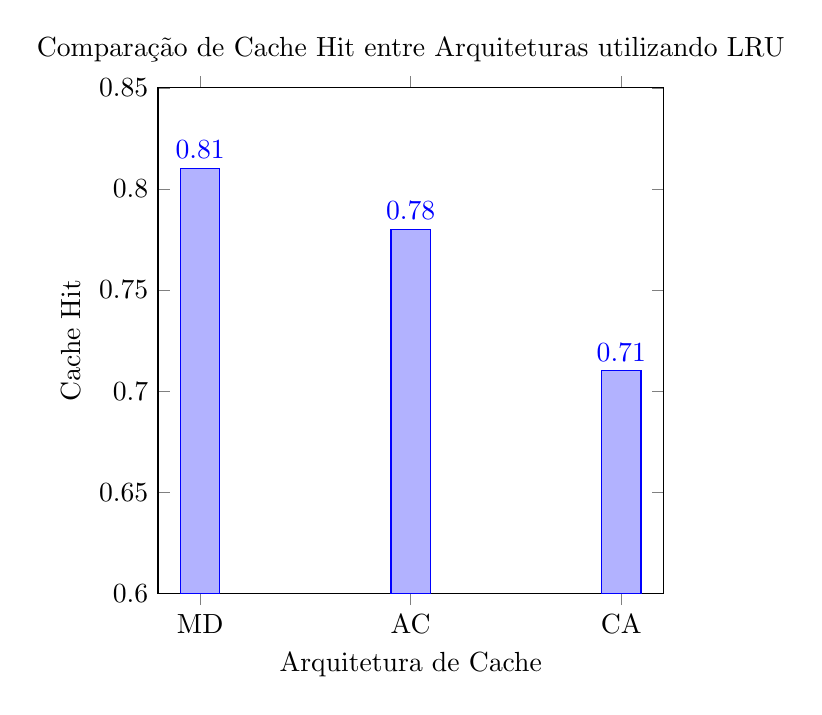
\begin{tikzpicture}
 \begin{axis}[
     ybar,
     symbolic x coords={MD, AC, CA},
     xtick=data,
     xlabel={Arquitetura de Cache},
     ylabel={Cache Hit},
     ymin=0.6, ymax=0.85,
     nodes near coords,
     bar width=0.5cm,
     width=8cm,
     height=8cm,
     title={Comparação de Cache Hit entre Arquiteturas utilizando LRU},
 ]
 % Dados do gráfico
 \addplot coordinates {
     (MD, 0.81)
     (AC, 0.78)
     (CA, 0.71)
 };
 \end{axis}
\end{tikzpicture}

O método LRU (Least Recently Used) é a política de substituição utilizada em memória cache (e também em outros campos da computação) que, ao ocorrer um miss, ou seja, um conflito no endereçamento da cache, remove o bloco que não foi utilizado a mais tempo. Um dos problemas dessa política é que nescessita o controle de quais blocos foram recentemente utilizados.

Os testes envolvendo a política LRU mostram que o desempenho é superior na arquitetura de mapeamento direto, porém bem próximo a eficácia da arquitetura associativa por conjunto. A arquitetura mais prejudicada pela política é a Completamente Associativa.

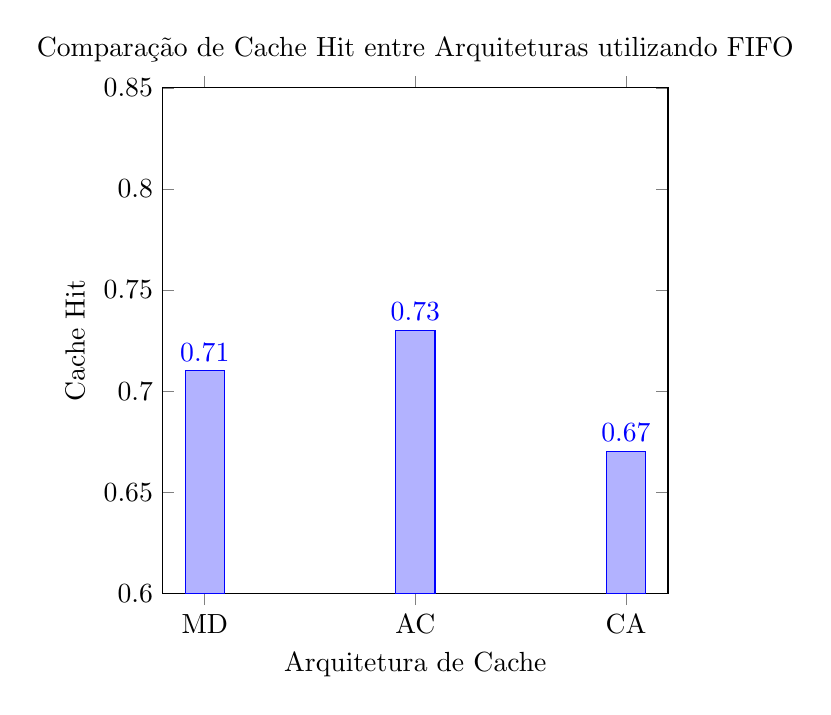
\begin{tikzpicture}
 \begin{axis}[
     ybar,
     symbolic x coords={MD, AC, CA},
     xtick=data,
     xlabel={Arquitetura de Cache},
     ylabel={Cache Hit},
     ymin=0.6, ymax=0.85,
     nodes near coords,
     bar width=0.5cm,
     width=8cm,
     height=8cm,
     title={Comparação de Cache Hit entre Arquiteturas utilizando FIFO},
 ]
 % Dados do gráfico
 \addplot coordinates {
     (MD, 0.71)
     (AC, 0.73)
     (CA, 0.67)
 };
 \end{axis}
\end{tikzpicture}

A política de substituição FIFO (First in First out) basea-se na ideia de Filas, onde o primeiro objeto a entrar é o primeiro a sair. Em resumo, os blocos são substituídos com base em sua ordem de chegada, o que nem sempre é ideal pois pode prejudicar a exploração da localidade espacial na memória cache.

Como resultado, é possível obersar que o método tem resultados próximos em todas as arquiteturas. Ao comparar os resultados das duas políticas analisadas nessa seção, é possível observar que a política LRU é substancialmente mais eficiente do que a política FIFO.

A constatação se deve ao fato de que a política LRU explora de forma mais eficiente os conceitos de localidade temporal e espacial, visto que só remove blocos que não estão sendo utilizados a algum tempo, enquanto a política FIFO remove o bloco independente se tiver sido utilizado recentemente ou não.

\section{Conclusão}
Uma cache real de alto desempenho deve conseguir obter um cache hit em torno de 0,9. Ou seja, de 10 buscas de dados/instruções na memória, 9 devem estar localizados na cache. Para alcançar bons resultados é preciso explorar a localidade temporal e espacial, conceitos teóricos da computação já citados anteriormente. 

Através de 4 cenários de testes diferentes, foi possível observar a sensibilidade da memória cache aos seguintes parâmetros: tamanho do bloco, tamanho do conjunto, tipo de organização e políticas de substituição.

A partir desses testes a primeira observação possível é que a memória é extremamente sensível ao tamanho dos blocos e da política de substituição. Quanto maior o tamanho do bloco, pior é a performance da cache pois o aumento desses dois parâmetros interfere diretamente no número de linhas da memória, diminuindo a quantidade de espaços possíveis para armazenar diferentes informações. Já a política de substituição tem impacto direto no cache hit, visto que, as políticas que ignoram os princípios da localidade, como a política FIFO, fazem com que o mesmo bloco seja removido e adicionado diversas vezes na cache.

O tamanho do conjunto também é um fator que pode atrapalhar o desempenho da memória, caso não seja pensado de maneira adequada. Isso ocorre pois, após um certo número de conjuntos, a associatividade é prejudicada.

Explorando as políticas de substituição, é possível concluir também que, para a política LRU, a arquitetura com melhor desempenho é a de Mapeamento Direto, enquanto a pior é a Completamente Associativa. Já na política FIFO, a arquitetura associativa por conjunto se sobresai.

Visando um cache hit em torno de 0,9, é possível concluir que as melhores combinações de parâmetros para explorar a eficiência máxima da memória, e consequentemente explorar ao máximo os princípios de localidade seriam memórias com mapeamento direto ou associativas por conjunto com blocos em torno de 64 Bytes e com política de substituição LRU, para uma memória cache de 256 Bytes e uma memória principal de 1024 Bytes. 

Além dos componentes explorados nesse trabalho, ainda existem muitos outros fatores que podem interferir na performance da cache, como o tamanho da palavra, tamanho da memória, entre outros.

\begin{thebibliography}{00}

\bibitem{patterson2017} D. A. Patterson and J. L. Hennessy, \textit{Organização e Projeto de Computadores: Interface Hardware/Software}, 4th ed. Rio de Janeiro: Elsevier, 2017.

\bibitem{amnesia1} F. R. Silva, M. C. Silveira, and J. P. Lima, "Aprendendo Hierarquia de Memória e a Exploração das Localidades Espacial e Temporal com o Simulador Amnesia," in \textit{Anais do Congresso Brasileiro de Informática na Educação (CBIE)}, vol. 8, pp. 105–112, 2020.

\bibitem{amnesia2} F. R. Silva, M.. Silveira, and J. P. Lima, "Amnesia: um Objeto de Aprendizagem para o Ensino de Hierarquia de Memória," in \textit{Revista Brasileira de Informática na Educação}, vol. 28, no. 2, pp. 75–88, 2021.

\bibitem{unesp_cache} J. R. Souza and M. T. Oliveira, "Avanços na Arquitetura de Memória Cache," UNESP - IBILCE, São José do Rio Preto, SP, Brasil, 2019. Disponível em: \url{https://www.ibilce.unesp.br}

\end{thebibliography}

\end{document}
